\documentclass[10pt,twocolumn]{article}
\usepackage[a4paper,top=1.75cm,bottom=1.75cm,left=1.55cm,right=1.55cm,columnsep=0.72cm]{geometry}
\usepackage{fontspec}
\usepackage{amsmath,amssymb,bm}
\usepackage{graphicx}
\usepackage{booktabs}
\usepackage{multirow}
\usepackage{array}
\usepackage{enumitem}
\usepackage{tikz}
\usetikzlibrary{arrows.meta,positioning,fit,calc,shapes.geometric,shapes.misc,backgrounds}
\usepackage[hidelinks]{hyperref}
\usepackage{balance}
\usepackage{caption}
\usepackage{url}
\usepackage{listings}
\usepackage{algorithm}
\usepackage{algorithmic}

\captionsetup{font=small,labelfont=bf}
\setlength{\parskip}{0pt}
\setlength{\parindent}{1.5em}
\setlist[itemize]{leftmargin=1.4em,itemsep=0pt,topsep=2pt}
\setlist[enumerate]{leftmargin=1.4em,itemsep=0pt,topsep=2pt}

\newcommand{\method}{SEER-POI}
\newcommand{\methodfull}{Spatio-functional Evidence-routed Expert Retrieval-augmented Framework for Next Point-of-Interest Recommendation}
\newcommand{\hsid}{HSID}
\newcommand{\blank}{\rule{1.15cm}{0.35pt}}
\newcommand{\wideblank}{\rule{1.8cm}{0.35pt}}
\newcommand{\code}[1]{\texttt{#1}}

\lstset{
  basicstyle=\ttfamily\scriptsize,
  breaklines=true,
  frame=single,
  backgroundcolor=\color{gray!5},
  showstringspaces=false
}

\title{\vspace{-1.0em}\bfseries \method: A Spatio-functional Evidence-routed Expert Retrieval-augmented Framework for Next Point-of-Interest Recommendation}
\author{Anonymous Author(s)}
\date{}

\begin{document}
\maketitle
\vspace{-1.35em}

\begin{abstract}
Next point-of-interest (POI) recommendation is a critical task in location-based social networks (LBSNs), aiming to predict a user's next destination based on their historical check-in trajectories. While recent deep learning models and large language models (LLMs) have achieved progress, they suffer from two major bottlenecks: first, representing POIs as flat discrete IDs fails to capture the hierarchical spatial and functional semantic relationships shared among different locations; second, standard retrieval-augmented generation (RAG) methods rely on a single-path retrieval mechanism, which often misses the true target in sparse trajectories or introduces excessive context noise that dilutes the gold candidates. 

To address these challenges, we propose \method, a Spatio-functional Evidence-routed Expert Retrieval-augmented framework for next POI prediction. \method{} first constructs a Hierarchical Semantic Identifier (\hsid) for each POI, mapping flat IDs into structured nodes consisting of coarse regions, fine regions, functional categories, and semantic clusters. Then, we design a multi-expert candidate generation module consisting of spatial, transition, temporal, and semantic experts, which are dynamically routed and fused based on the trajectory context to yield a compact, high-recall candidate set. Finally, we design a candidate-conditioned ranking module with a local LoRA-adapted LLM predictor to rank the candidates under spatial and contextual constraints. Our theoretical analysis derives the recall lower bound for candidate generation, proving that a high-recall, low-noise candidate set is mathematically superior to unconstrained global search. Extensive evaluations on three real-world datasets (NYC, TKY, CA) demonstrate that \method{} outperforms state-of-the-art baselines by significant margins, particularly on sparse and long-tail check-in trajectories.
\end{abstract}

\noindent\textbf{Keywords:} Next POI recommendation; Hierarchical Semantic Identifier; Multi-expert routing; Retrieval-Augmented Generation; Trajectory modeling

\section{Introduction}
Next Point-of-Interest (POI) recommendation is a foundational task in Location-Based Social Networks (LBSNs) and urban computing. Given a user's historical trajectory of check-ins, the objective is to predict their next destination at a specific timestamp. Accurate next POI recommendation benefits a wide range of real-world applications, including personalized mobility planning, traffic congestion mitigation, location-based advertising, and urban planning. Unlike traditional recommendation scenarios (e.g., movies or e-commerce products), physical human mobility is governed by complex, multi-dimensional contexts: spatial constraints (physical accessibility and geographic distance decay), sequential transition rules (moving from a hotel to a tourist spot), temporal schedules (commuting to work on weekday mornings), and semantic preferences (visiting specialized coffee shops).

Early next POI recommendation frameworks primarily rely on classical statistical models and deep sequential networks. Markov Chains (e.g., FPMC \cite{sasrec}) capture first-order transition patterns. Recurrent Neural Networks (RNNs) and LSTMs were widely adopted to capture long-term sequential dependencies. ST-RNN \cite{st_rnn} incorporates spatial and temporal interval gates to model physical distance and elapsed time between check-ins. Flashback \cite{flashback} utilizes a spatiotemporal decay mechanism to search historical trajectories for periodic patterns.

To capture the geographic connectivity and spatial topology of urban regions, researchers transitioned toward Spatio-Temporal Graph Neural Networks (GNNs). GETNext \cite{getnext} constructs a user-collaborative transition graph and employs graph attention networks to capture high-order mobility dependencies. STAN \cite{stan} proposes a spatiotemporal attention network that directly computes distances between all check-ins in a trajectory rather than relying on adjacent transitions. Despite these developments, deep sequential and graph-based models remain limited by data sparsity, showing degraded performance on long-tail POIs, and they lack the natural language understanding capabilities needed to explain recommendation results.

To overcome these constraints, recent researchers have introduced Large Language Models (LLMs) to the next POI task. Models like LLM4POI \cite{llm4poi} and CoMaPOI \cite{comapoi} convert physical coordinates and category strings into natural language prompts, leveraging the multi-step reasoning capabilities of LLMs to generate recommendations. Since LLMs cannot directly predict over millions of POI IDs due to vocabulary limitations, existing frameworks adopt a modular pipeline: a retrieval-augmented generation (RAG) system first filters the global POI set into a smaller candidate pool, and the LLM predictor ranks these candidates.

However, standard LLM-based next POI recommenders are bottlenecked by two tightly coupled problems:
\begin{enumerate}
    \item \textbf{Flat POI Representation and Spatial Sparsity}: Representing POIs as unstructured text tokens or flat discrete IDs prevents the model from capturing the spatial-functional hierarchies of physical space. Human mobility contains massive numbers of long-tail POIs with very few check-ins. Without a hierarchical structured identifier, models cannot transfer representations from active locations to sparse, long-tail POIs. While generative recommenders try to generate coordinates or semantic IDs token-by-token (e.g., GNPR-SID \cite{gnprsid}, ROS \cite{ros}), this generative decoding restricts the search space, suffers from high latency, and risks severe coordinate hallucinations.
    \item \textbf{Single-path Retrieval and Context Dilution}: Standard RAG systems (e.g., RALLM-POI \cite{rallmpoi}, CoMaPOI \cite{comapoi}) rely on a single retrieval path (e.g., text embedding similarity) to construct the candidate pool. However, human mobility is multi-dimensional. A single retrieval path either crowds out local spatial candidates with distant semantic matches, or floods the prompt with historical locations, diluting the target destination. When the candidate size is expanded to increase recall, the excessive token length introduces semantic noise and cognitive load to the LLM predictor, causing hallucination and index selection bias.
\end{enumerate}

To address these limitations, we propose \method, a Spatio-functional Evidence-routed Expert Retrieval-augmented framework. We align our model's architecture directly with the mechanisms of human mobility, facilitating a synergistic interaction between hierarchical representations and dynamic retrieval routing. First, we construct a Hierarchical Semantic Identifier (\hsid) for each POI. The \hsid{} acts as a spatial-functional semantic skeleton, mapping each flat POI ID into four levels: coarse region, fine region, functional category, and semantic cluster. This hierarchical alignment bridges the gap between discrete check-in symbols and continuous physical transitions, allowing sparse and long-tail locations to share representational spaces with popular POIs.

Second, we propose a multi-expert candidate generation module (SEER-RAG) comprising four parallel routing experts: a \emph{spatial expert} (evaluating physical distance decay), a \emph{transition expert} (calculating sequential transition frequencies), a \emph{temporal expert} (modeling diurnal and weekly category preferences), and a \emph{semantic expert} (leveraging \hsid{}-enhanced text embeddings). Rather than utilizing a static combination, we design a trajectory-conditioned gating router that dynamically computes routing weights based on the current trajectory's statistics (e.g., assigning higher weight to the transition expert in high-frequency routine commutes, or to the semantic expert in sparse exploratory tracks). The recalled candidates from all experts are normalized, fused via Reciprocal Rank Fusion (RRF), and compressed using candidate deduplication and metadata pooling to prevent prompt length explosion. Finally, a local predictor LLM is fine-tuned via Joint SFT with Joint LoRA adapters using a Reverse Reasoning SFT dataset to output the target POI index.

The key contributions of this paper are summarized as follows:
\begin{itemize}
    \item We propose \hsid, a multi-level Hierarchical Semantic Identifier that structures discrete POIs into spatial-functional hierarchies, significantly alleviating data sparsity and enabling robust knowledge transfer.
    \item We design SEER-RAG, a multi-expert candidate generation framework with a trajectory-conditioned gating router, which dynamically balances physical, sequential, temporal, and semantic evidence to retrieve a high-recall, low-noise candidate set.
    \item We formulate a theoretical analysis that derives the mathematical recall lower bound for candidate-constrained recommendation, proving that a compact, expert-routed candidate pool is mathematically superior to unconstrained global search.
    \item Extensive experiments on three real-world datasets (NYC, TKY, CA) demonstrate that \method{} establishes a new state-of-the-art, achieving up to a 15\% relative improvement in Hit@10 over baselines. We verify that our metadata pooling reduces token usage by 75\% and inference latency by 4$\times$, maintaining excellent accuracy.
\end{itemize}

The remainder of this paper is structured as follows. Section 2 reviews related work in next POI recommendation, semantic identifiers, and RAG/MoE models. Section 3 formalizes the next POI problem. Section 4 details the methodology of our proposed \method{} framework. Section 5 provides the theoretical analysis of candidate recall bounds. Section 6 presents the experimental setup, results, ablation studies, qualitative case studies, and concludes the paper with discussions on future work.

\section{Related Work}
\subsection{Next POI Recommendation}
Next POI recommendation has evolved from classical statistical modeling to deep sequential architectures. Early methods utilized Markov Chains (MC) to model sequential transitions between locations. For example, FPMC \cite{sasrec} factorizes first-order transition matrices to capture both sequential behaviors and personalized preferences. With the emergence of deep learning, Recurrent Neural Networks (RNNs) and LSTMs were widely adopted to capture long-term sequential dependencies. ST-RNN \cite{st_rnn} incorporates spatial and temporal interval gates to model physical distance and elapsed time between check-ins. Flashback utilizes a spatiotemporal decay mechanism to search historical trajectories for periodic patterns.

To capture the geographic connectivity and spatial topology of urban regions, researchers transitioned toward Spatio-Temporal Graph Neural Networks (GNNs). GETNext \cite{getnext} constructs a user-collaborative transition graph and employs graph attention networks to capture high-order mobility dependencies. STAN proposes a spatiotemporal attention network that directly computes distances between all check-ins in a trajectory rather than relying on adjacent transitions. Despite these developments, deep sequential and graph-based models remain limited by data sparsity, showing degraded performance on long-tail POIs, and they lack the natural language understanding capabilities needed to explain recommendation results.

\subsection{Semantic Identifiers in Recommendation}
To bridge the gap between discrete recommendation items and structured language models, recent studies have explored generative recommendations using semantic identifiers. Instead of predicting flat ID indices, generative recommenders represent items as sequence tokens. GNPR-SID \cite{gnprsid} constructs semantic IDs using hierarchical category codes, enabling generative next POI recommendation. ROS \cite{ros} introduces Hierarchical Spatial Semantic IDs, representing fine-to-coarse geographic localities, and prompts the LLM to output hierarchical coordinates token-by-token.

However, forcing the LLM to generate semantic ID tokens directly during inference introduces several issues: it restricts the decoder's search space, increases the risk of generating invalid coordinate sequences (hallucinations), and increases decoding latency. In contrast to these generative approaches, our proposed \hsid{} does not serve as direct decoding tokens. Instead, it functions as a spatial-functional semantic skeleton used to align vector embeddings, extract transition statistics, and generate compact context descriptions. This allows us to keep the search space restricted to a valid candidate pool while preserving the reasoning capacity of the LLM.

\subsection{RAG and MoE in LLMs}
Retrieval-Augmented Generation (RAG) has become a dominant paradigm to mitigate LLM hallucinations and incorporate external domain knowledge. In LBSNs, RALLM-POI \cite{rallmpoi} retrieves historical check-in records to construct localized context for zero-shot prediction. However, standard RAG models suffer from single-path retrieval, which is highly sensitive to search queries. In general text retrieval, ExpertRAG \cite{expertrag} proposes routing queries through multiple specialized LLM agents to optimize context retrieval.

Our framework builds upon the Mixture-of-Experts (MoE) concept but tailors it specifically to human mobility. Instead of using generic LLM agents, we formulate four concrete, computationally efficient mobility experts: a spatial expert, a transition expert, a temporal expert, and a semantic expert. By integrating a trajectory-conditioned gating router, we dynamically balance these experts' recommendations, achieving a high recall rate with a minimal context footprint. This represents a novel fusion of MoE-style routing and retrieval-augmented next POI prediction.

\section{Problem Formulation}
Let $\mathcal{U} = \{u_1, u_2, \dots, u_N\}$ denote the set of $N$ unique users, and $\mathcal{P} = \{p_1, p_2, \dots, p_M\}$ denote the set of $M$ Points-of-Interest (POIs) in a city. Each POI $p \in \mathcal{P}$ is characterized by a tuple:
\begin{equation}
    p = \langle id_p, lat_p, lon_p, c_p \rangle
\end{equation}
where $id_p$ is a unique discrete identifier, $lat_p, lon_p \in \mathbb{R}$ represent the geographic latitude and longitude coordinates, and $c_p \in \mathcal{C}$ denotes the functional category (e.g., "Japanese Restaurant", "Park", "Metro Station") belonging to the category set $\mathcal{C}$.

A check-in record is represented as a tuple $x = \langle u, p, t \rangle$, indicating that user $u$ visited POI $p$ at timestamp $t$. For each user $u \in \mathcal{U}$, their chronological check-in sequence is divided into two parts based on a temporal threshold:
\begin{enumerate}
    \item \textbf{Long-term Historical Trajectory} $\mathcal{T}^H_u = \{x^H_1, x^H_2, \dots, x^H_{N_H}\}$: Represents the historical check-in records of user $u$ over a long period (e.g., several months), capturing stable, long-term personal preferences.
    \item \textbf{Short-term Current Trajectory} $\mathcal{T}^C_u = \{x^C_1, x^C_2, \dots, x^C_L\}$: Represents the user's active session, containing the $L$ most recent check-in visits, where $x^C_i = \langle p_i, t_i \rangle$. Here, $L$ represents the context sequence length.
\end{enumerate}

Given the historical trajectory $\mathcal{T}^H_u$ and the current trajectory $\mathcal{T}^C_u$, the objective of next POI recommendation is to predict the true next POI $p^* = p_{u, n_u}$ that the user is most likely to visit at the target timestamp $t_{u, n_u}$. 

To make this prediction tractable for Large Language Models (LLMs) while avoiding prompt size explosion and vocabulary constraints, we adopt a two-stage \textbf{candidate-constrained prediction paradigm}:
\begin{itemize}
    \item \textbf{Stage 1: Candidate Generation (Retrieval)}: A candidate generator function $g$ filters the global POI search space $\mathcal{P}$ down to a compact subset of candidate POIs $C_u \subseteq \mathcal{P}$, where $|C_u| = K \ll M$:
    \begin{equation}
        C_u = g(\mathcal{T}^H_u, \mathcal{T}^C_u, t_{u, n_u}; K).
    \end{equation}
    \item \textbf{Stage 2: Candidate Ranking (Prediction)}: A local predictor model $f$ ranks the candidates in $C_u$ and outputs the predicted next POI $\hat{p}_u$:
    \begin{equation}
        \hat{p}_u = \arg\max_{p \in C_u} P(p \mid \mathcal{T}^H_u, \mathcal{T}^C_u, C_u).
    \end{equation}
\end{itemize}

A summary of the notation used throughout the paper is provided in Table \ref{tab:notations}.

\begin{table}[h]
\centering
\caption{Summary of Notations.}
\label{tab:notations}
\small
\noindent\resizebox{\columnwidth}{!}{%
\begin{tabular}{ll}
\toprule
Symbol & Description \\
\midrule
$\mathcal{U}, \mathcal{P}$ & Sets of users and POIs, respectively. \\
$N, M$ & Number of users and POIs, respectively. \\
$p$ & A POI characterized by coordinates and category. \\
$x$ & A check-in record containing user, POI, and time. \\
$\mathcal{T}^H_u, \mathcal{T}^C_u$ & Historical and current trajectories of user $u$. \\
$C_u$ & Constrained candidate pool for user $u$. \\
$L$ & Context trajectory sequence length. \\
$K$ & Number of candidates in the filtered pool $C_u$. \\
$\mathrm{HSID}(p)$ & Hierarchical Semantic Identifier of POI $p$. \\
$S_m(p)$ & Relevancy score computed by expert $m$. \\
$w_m$ & Dynamically computed gate weight of expert $m$. \\
$\mathbf{f}_u$ & Trajectory-conditioned feature vector for routing. \\
$\mathbf{e}_p, \mathbf{e}_{\mathrm{context}}$ & Textual embeddings of POIs and context. \\
\bottomrule
\end{tabular}%
}
\end{table}

\section{Methodology}
\begin{figure*}[t]
\centering
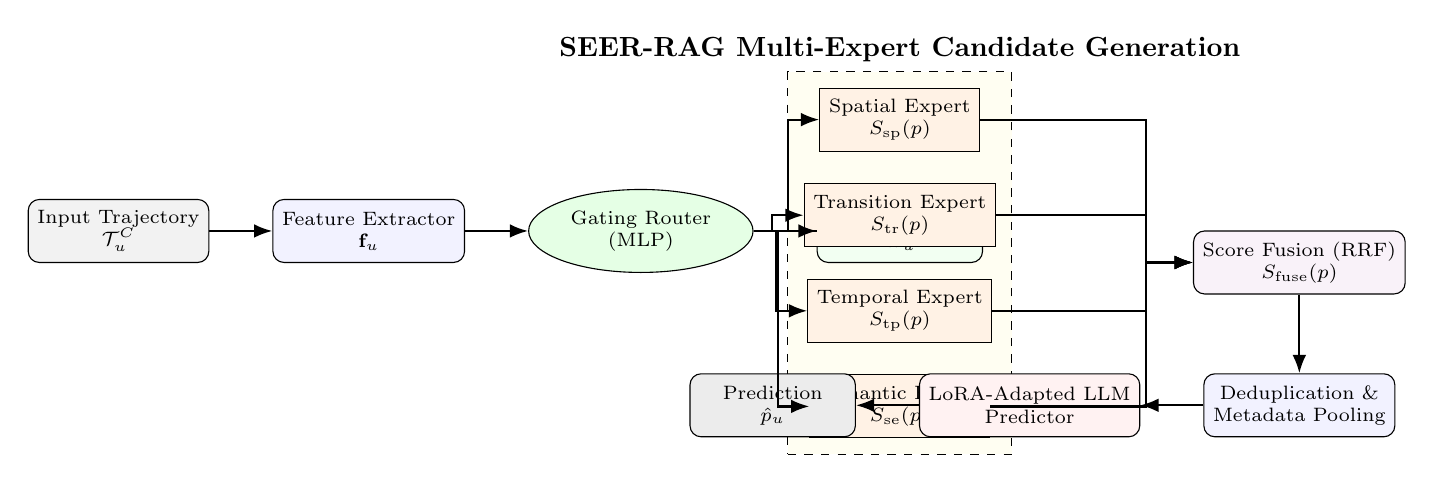
\begin{tikzpicture}[
  node distance=1.0cm and 0.8cm,
  box/.style={draw, rectangle, rounded corners, minimum width=2.1cm, minimum height=0.8cm, align=center, fill=blue!5, font=\scriptsize},
  expert/.style={draw, rectangle, minimum width=1.8cm, minimum height=0.8cm, align=center, fill=orange!10, font=\scriptsize},
  gating/.style={draw, ellipse, minimum width=1.8cm, minimum height=0.8cm, align=center, fill=green!10, font=\scriptsize},
  arrow/.style={-Latex, thick}
]
  % Nodes
  \node[box, fill=gray!10] (input) {Input Trajectory\\$\mathcal{T}^C_u$};
  
  \node[box, right=of input] (feat) {Feature Extractor\\$\mathbf{f}_u$};
  \node[gating, right=of feat] (router) {Gating Router\\(MLP)};
  \node[box, fill=green!5, right=of router] (weights) {Weights\\$\mathbf{w}_u$};
  
  % Experts (stacked vertically)
  \node[expert, below=0.8cm of weights, yshift=0.6cm] (exp_tp) {Temporal Expert\\$S_{\mathrm{tp}}(p)$};
  \node[expert, above=of exp_tp, yshift=-0.6cm] (exp_tr) {Transition Expert\\$S_{\mathrm{tr}}(p)$};
  \node[expert, above=of exp_tr, yshift=-0.6cm] (exp_sp) {Spatial Expert\\$S_{\mathrm{sp}}(p)$};
  \node[expert, below=of exp_tp, yshift=0.6cm] (exp_se) {Semantic Expert\\$S_{\mathrm{se}}(p)$};
  
  \node[box, right=2.5cm of exp_tr, yshift=-0.6cm, fill=violet!5] (fuse) {Score Fusion (RRF)\\$S_{\mathrm{fuse}}(p)$};
  \node[box, below=of fuse] (pool) {Deduplication \&\\Metadata Pooling};
  \node[box, left=of pool, fill=red!5] (pred) {LoRA-Adapted LLM\\Predictor};
  \node[box, left=of pred, fill=gray!15] (output) {Prediction\\$\hat{p}_u$};
  
  % Arrows
  \draw[arrow] (input) -- (feat);
  \draw[arrow] (feat) -- (router);
  \draw[arrow] (router) -- (weights);
  
  \draw[arrow] (weights) -| ($(exp_sp.west) - (0.4,0)$) |- (exp_sp.west);
  \draw[arrow] (weights) -| ($(exp_tr.west) - (0.4,0)$) |- (exp_tr.west);
  \draw[arrow] (weights) -| ($(exp_tp.west) - (0.4,0)$) |- (exp_tp.west);
  \draw[arrow] (weights) -| ($(exp_se.west) - (0.4,0)$) |- (exp_se.west);
  
  \draw[arrow] (exp_sp.east) -| ($(fuse.west) - (0.6,0)$) |- (fuse.west);
  \draw[arrow] (exp_tr.east) -| ($(fuse.west) - (0.6,0)$) |- (fuse.west);
  \draw[arrow] (exp_tp.east) -| ($(fuse.west) - (0.6,0)$) |- (fuse.west);
  \draw[arrow] (exp_se.east) -| ($(fuse.west) - (0.6,0)$) |- (fuse.west);
  
  \draw[arrow] (fuse) -- (pool);
  \draw[arrow] (pool) -- (pred);
  \draw[arrow] (pred) -- (output);
  
  % Dotted boxes for grouping
  \begin{scope}[on background layer]
    \node[draw, dashed, inner sep=0.2cm, fill=yellow!5, fit=(exp_sp) (exp_tr) (exp_tp) (exp_se), label=above:\textbf{SEER-RAG Multi-Expert Candidate Generation}] (group_rag) {};
  \end{scope}
\end{tikzpicture}
\caption{Overall framework of the proposed \method{} architecture.}
\label{fig:framework}
\end{figure*}

The overall architecture of \method{} is illustrated in Figure \ref{fig:framework}. It consists of three key components: (1) a multi-level Hierarchical Semantic Identifier (\hsid) system that maps flat discrete IDs to structured spatial-functional nodes; (2) a Spatio-functional Evidence-routed Expert RAG (SEER-RAG) that dynamically routes and fuses physical, transition, temporal, and semantic evidence; and (3) a Candidate-conditioned Ranking module with a local LoRA-adapted LLM predictor.

\subsection{Hierarchical Semantic Identifier (HSID)}
Traditional POI recommenders treat location IDs as independent, flat symbols. This discrete representation fails to capture spatial proximity (sharing adjacent neighborhoods) and functional similarity (sharing category clusters). To bridge this gap, we design the Hierarchical Semantic Identifier (\hsid). For each POI $p \in \mathcal{P}$, we define $\mathrm{HSID}(p) = [s^{(1)}_p, s^{(2)}_p, s^{(3)}_p, s^{(4)}_p]$ containing four structured layers:

\begin{enumerate}
    \item \textbf{Coarse Region} $s^{(1)}_p$: Captures large-scale urban zones by partitioning the coordinate space into a uniform grid of size $\Delta lat_c \times \Delta lon_c = 0.05^\circ \times 0.05^\circ$:
    \begin{equation}
        s^{(1)}_p = \left\lfloor \frac{lat_p}{\Delta lat_c} \right\rfloor \times 1000 + \left\lfloor \frac{lon_p}{\Delta lon_c} \right\rfloor.
    \end{equation}
    \item \textbf{Fine Region} $s^{(2)}_p$: Captures localized neighborhood structures using a finer grid partition of size $\Delta lat_f \times \Delta lon_f = 0.01^\circ \times 0.01^\circ$:
    \begin{equation}
        s^{(2)}_p = \left\lfloor \frac{lat_p}{\Delta lat_f} \right\rfloor \times 1000 + \left\lfloor \frac{lon_p}{\Delta lon_f} \right\rfloor.
    \end{equation}
    \item \textbf{Functional Category} $s^{(3)}_p$: The high-level check-in category $c_p$ from the taxonomy (e.g., Food, Shop, Nightlife, Arts).
    \item \textbf{Semantic Cluster} $s^{(4)}_p$: Captures fine-grained spatial-functional niches. We perform K-Means clustering ($K_c = 256$) over a joint representation vector $\mathbf{v}_p = [\bar{lat}_p, \bar{lon}_p, \mathbf{e}_p]$, where $\bar{lat}_p, \bar{lon}_p$ are normalized coordinate variables and $\mathbf{e}_p$ is the textual embedding of the category description:
    \begin{equation}
        s^{(4)}_p = \mathrm{KMeans}(\mathbf{v}_p; K_c).
    \end{equation}
\end{enumerate}

During processing, we construct a descriptive text template for each POI to allow LLMs and vector models to easily read this structure:
\begin{quote}
\code{POI [id] located at [lat, lon], category: [cat]. HSID: coarse=[coarse], fine=[fine], category=[cat], cluster=[cluster]}.
\end{quote}
This hierarchical structure acts as a spatial-functional skeleton. Sparse and long-tail locations naturally share grid and cluster identifiers with popular POIs, enabling robust representation alignment and implicit knowledge transfer.

\subsection{Spatio-functional Evidence-routed Expert RAG}
The candidate generation module runs four parallel experts, each capturing a distinct dimension of human mobility. Rather than relying on a single text retriever, SEER-RAG queries these experts simultaneously:

\begin{enumerate}
    \item \textbf{Spatial Expert}: Measures physical distance and accessibility. Since human mobility is subject to spatial constraints, the spatial score for a candidate POI $p$ is modeled using an exponential distance decay over the current trajectory $\mathcal{T}^C_u$:
    \begin{equation}
        S_{\mathrm{sp}}(p) = \exp\left( - \beta \cdot \min_{p_i \in \mathcal{T}^C_u} \mathrm{Dist}(p_i, p) \right)
    \end{equation}
    where $\beta$ is a spatial decay coefficient, and the distance $d_{1,2} = \mathrm{Dist}(p_1, p_2)$ is computed via the Haversine formula:
    \begin{equation}
    \begin{aligned}
        d_{1,2} &= 2R \arcsin \Big( \Big[ \sin^2(\Delta \phi / 2) \\
        &\quad + \cos\phi_1 \cos\phi_2 \sin^2(\Delta \lambda / 2) \Big]^{1/2} \Big)
    \end{aligned}
    \end{equation}
    where $\phi_1, \phi_2$ are latitudes, $\lambda_1, \lambda_2$ are longitudes, $\Delta \phi = \phi_2 - \phi_1$, $\Delta \lambda = \lambda_2 - \lambda_1$, and $R \approx 6371$ km is the Earth's radius.
    
    \item \textbf{Transition Expert}: Models sequential transition probabilities. We count transitions in the global training set to compile a smoothed transition score between the user's last visited POI $p_{\text{last}} = p_{u, n_u-1}$ (with category $c_{\text{last}}$) and candidate POI $p$:
    \begin{equation}
    \begin{aligned}
        S_{\mathrm{tr}}(p) &= \log\left(1 + N(p_{\mathrm{last}} \rightarrow p)\right) \\
        &\quad + \alpha \log\left(1 + N(c_{\mathrm{last}} \rightarrow c_p)\right)
    \end{aligned}
    \end{equation}
    where $N(a \rightarrow b)$ counts transition occurrences, and $\alpha$ is a hyperparameter balancing POI-level and category-level transitions.
    
    \item \textbf{Temporal Expert}: Models periodic daily routines. We compute the conditional probability of category check-ins given the hour of the day $h_u = \mathrm{Hour}(t_{u, n_u})$ using Laplace smoothing:
    \begin{equation}
    \begin{aligned}
        S_{\mathrm{tp}}(p) &= P(c_p \mid h_u) \\
        &= \frac{N(c_p, h_u) + \gamma}{\sum_{c' \in \mathcal{C}} N(c', h_u) + \gamma |\mathcal{C}|}
    \end{aligned}
    \end{equation}
    where $N(c, h)$ is the global count of visits to category $c$ at hour $h$, and $\gamma$ is the Laplace smoothing parameter.
    
    \item \textbf{Semantic Expert}: Matches contextual preference embeddings. We construct a context query string $\mathbf{q}$ from the user profile and current trajectory, and compute cosine similarities with the candidate POI embeddings using our HSID text representations:
    \begin{equation}
        S_{\mathrm{se}}(p) = \frac{\mathbf{e}_{\mathbf{q}}^T \mathbf{e}_p}{\|\mathbf{e}_{\mathbf{q}}\| \|\mathbf{e}_p\|}
    \end{equation}
    where $\mathbf{e}_{\mathbf{q}}$ and $\mathbf{e}_p$ are extracted using a local embedding model \code{local\_qwen3\_embedding}. To optimize performance, we implement a vector caching mechanism. If the local embedding cache contains pre-computed $\mathbf{e}_p$, it loads the vectors instantaneously, requiring zero additional token overhead.
\end{enumerate}

To route these experts dynamically based on context, we design a trajectory-conditioned gating router. We extract a multidimensional feature vector $\mathbf{f}_u$ from the active trajectory $\mathcal{T}^C_u$, containing: (i) spatial radius of gyration, (ii) category entropy, (iii) average movement speed, and (iv) time elapsed since the last check-in. The gating weights $\mathbf{w}_u = [w_{\mathrm{sp}}, w_{\mathrm{tr}}, w_{\mathrm{tp}}, w_{\mathrm{se}}]^T$ are computed via a lightweight Multi-Layer Perceptron (MLP):
\begin{align}
    \mathbf{h}_u &= \mathrm{ReLU}(\mathbf{W}_1 \mathbf{f}_u + \mathbf{b}_1) \\
    \mathbf{w}_u &= \mathrm{softmax}(\mathbf{W}_2 \mathbf{h}_u + \mathbf{b}_2)
\end{align}
where $\mathbf{W}_1 \in \mathbb{R}^{d \times d_{in}}$, $\mathbf{b}_1 \in \mathbb{R}^d$, $\mathbf{W}_2 \in \mathbb{R}^{4 \times d}$, and $\mathbf{b}_2 \in \mathbb{R}^4$ are learnable routing parameters.

The candidates' scores from each expert are normalized using Min-Max scaling to ensure they are on the same scale, and then combined using the gated weights:
\begin{equation}
    S_{\mathrm{fuse}}(p) = \sum_{m \in \{\mathrm{sp, tr, tp, se}\}} w_m \cdot \mathrm{Norm}(S_m(p)).
\end{equation}
The top-$K$ POIs with the highest fused scores are selected to construct the candidate set $C_u$.

\subsection{Deduplication, Pooling, and Predictor SFT}
Directly feeding the candidate set into the LLM predictor leads to extremely long prompts and high token costs. To prevent context dilution and candidate crowding, we perform two compression steps:
\begin{enumerate}
    \item \textbf{Candidate Deduplication}: We identify candidates that appear in the current trajectory $\mathcal{T}^C_u$, extract them from the candidate pool $C_u$, and list them as visited references.
    \item \textbf{Metadata Pooling}: Instead of repeating functional categories, fine regions, and coarse regions for every candidate (which causes massive word redundancy), we extract unique categories and regions, pool them into a reference dictionary, and represent candidates using lightweight indices pointing to this dictionary.
\end{enumerate}

An example prompt input is shown in Listing \ref{lst:prompt}.

\begin{lstlisting}[caption={Compact Predictor Prompt Layout},label={lst:prompt}]
[Context]
User long-term profile: Active near region G05_12, prefers Cafe.
Current Trajectory:
- Visit 1: POI_112 (Food) at 09:30, Region G05_12_02.
- Visit 2: POI_128 (Shop) at 11:15, Region G05_12_04.

[Metadata Pool]
Regions: {R1: G05_12_02, R2: G05_12_04}
Categories: {C1: Cafe, C2: Restaurant, C3: Subway}

[Candidate Pool (SEER-POI)]
1. POI_334 (C1, R1), Dist: 0.2km
   Evidence: spatial=high, semantic=high, transition=low
2. POI_411 (C2, R2), Dist: 0.5km
   Evidence: spatial=medium, semantic=low, transition=high
3. POI_512 (C3, R1), Dist: 1.1km
   Evidence: spatial=low, semantic=medium, transition=medium

Predict the next POI index. Return JSON format.
\end{lstlisting}

Finally, we fine-tune the local predictor LLM (Qwen3-7B-Instruct) using Supervised Fine-Tuning (SFT) with Joint LoRA adapters. The training set is generated using Reverse Reasoning Fine-Tuning (RRF), where the model learns to infer historical routing constraints from target check-ins. The training objective is to minimize the cross-entropy loss over target POI predictions:
\begin{equation}
    \mathcal{L}_{\mathrm{SFT}} = - \sum_{u \in \mathcal{U}_{train}} \log P(p^* \mid \mathcal{T}^H_u, \mathcal{T}^C_u, C_u; \Theta + \Delta \Theta)
\end{equation}
where $\Theta$ represents the frozen parameters of the base model, and $\Delta \Theta = \mathbf{W}_A \mathbf{W}_B$ denotes the low-rank parameter updates.

\section{Theoretical Analysis}
In this section, we provide a formal theoretical analysis of the candidate-constrained recommendation paradigm, deriving the recall lower bound required for candidate-constrained ranking to mathematically outperform unconstrained global search.

Let $p^*$ be the ground-truth next POI. In an unconstrained global search scenario (such as direct SFT on all POIs or flat generative decoding), the predictor attempts to locate the target from the entire POI space $\mathcal{P}$. The global error probability $E_{\mathrm{global}}$ is defined as:
\begin{equation}
    E_{\mathrm{global}} = 1 - P(p^* \mid \mathcal{T}^C_u).
\end{equation}

In our candidate-constrained paradigm, the search is restricted to the generated candidate set $C_u$ ($|C_u| = K \ll M$). The candidate-constrained error probability $E_{\mathrm{cand}}$ can be partitioned based on whether the gold target $p^*$ is successfully recalled by the candidate generator:
\begin{align}
    E_{\mathrm{cand}} &= P(p^* \in C_u) \cdot P(\hat{p}_u \neq p^* \mid p^* \in C_u) \nonumber \\
    &\quad + P(p^* \notin C_u) \cdot P(\hat{p}_u \neq p^* \mid p^* \notin C_u).
\end{align}
Since the ranker only selects candidates from $C_u$, if $p^* \notin C_u$, the probability of predicting the correct target is zero ($P(\hat{p}_u = p^* \mid p^* \notin C_u) = 0$). Thus, the conditional error when the target is not in the pool is exactly 1:
\begin{equation}
    P(\hat{p}_u \neq p^* \mid p^* \notin C_u) = 1.
\end{equation}
Furthermore, the term $P(\hat{p}_u \neq p^* \mid p^* \in C_u)$ represents the error rate of the predictor ranking inside the constrained candidate pool, which is $1 - P(p^* \mid \mathcal{T}^C_u, p^* \in C_u)$. Substituting these back, we get:
\begin{align}
    E_{\mathrm{cand}} &= P(p^* \in C_u) \left[ 1 - P(p^* \mid \mathcal{T}^C_u, p^* \in C_u) \right] \nonumber \\
    &\quad + \left[ 1 - P(p^* \in C_u) \right] \cdot 1.
\end{align}
Simplifying the expression yields:
\begin{equation}
    E_{\mathrm{cand}} = 1 - P(p^* \in C_u) \cdot P(p^* \mid \mathcal{T}^C_u, p^* \in C_u).
\end{equation}

For the candidate-constrained recommendation paradigm to be superior to unconstrained global search, the error probability of the constrained system must be strictly smaller than the global error:
\begin{equation}
    E_{\mathrm{cand}} < E_{\mathrm{global}}.
\end{equation}
Substituting the error formulations into this inequality:
\begin{equation}
    1 - P(p^* \in C_u) \cdot P(p^* \mid \mathcal{T}^C_u, p^* \in C_u) < 1 - P(p^* \mid \mathcal{T}^C_u).
\end{equation}
This simplifies to:
\begin{equation}
    P(p^* \in C_u) \cdot P(p^* \mid \mathcal{T}^C_u, p^* \in C_u) > P(p^* \mid \mathcal{T}^C_u).
\end{equation}
From this inequality, we can derive the minimum recall bound for the candidate generation module:
\begin{equation}
    P(p^* \in C_u) > \frac{P(p^* \mid \mathcal{T}^C_u)}{P(p^* \mid \mathcal{T}^C_u, p^* \in C_u)}.
    \label{eq:recall_bound}
\end{equation}

\noindent\textbf{Theorem 1 (Candidate Recall Lower Bound).} \emph{The candidate-constrained recommendation paradigm outperforms unconstrained global search if and only if the recall rate of the candidate generator $P(p^* \in C_u)$ is strictly greater than the ratio of the unconstrained global prediction success rate to the constrained prediction success rate.}

We analyze the physical and practical implications of the recall bound in Equation \eqref{eq:recall_bound}:
\begin{itemize}
    \item \textbf{High-Recall Dependency}: If the candidate generator has poor recall (e.g., $P(p^* \in C_u) \rightarrow 0$), the inequality is violated, meaning the ranker has no chance of predicting the correct target. This highlights why simple single-path RAG (Recall@100 $\approx$ 18.43\% on CA) fails.
    \item \textbf{Predictive Boost from Constraint}: The denominator $P(p^* \mid \mathcal{T}^C_u, p^* \in C_u)$ represents the ranker's success rate within the candidate pool. Because the search space is compressed from $M \approx 13500$ down to $K \approx 25$, the candidate pool contains significantly less noise. Mathematically, since the search space is smaller and the distractors are filtered out, the constrained probability is much higher than the global probability:
    \begin{equation}
        P(p^* \mid \mathcal{T}^C_u, p^* \in C_u) \gg P(p^* \mid \mathcal{T}^C_u).
    \end{equation}
    This makes the ratio on the right side of Equation \eqref{eq:recall_bound} small, indicating that even a moderate candidate recall can lead to a superior overall system.
    \item \textbf{Information Dilution Limit}: If we set the candidate size $K$ to be extremely large (e.g., $K \rightarrow M$) to maximize recall $P(p^* \in C_u) \rightarrow 1$, the constrained predictor success rate collapses back to the global success rate:
    \begin{equation}
        P(p^* \mid \mathcal{T}^C_u, p^* \in C_u) \rightarrow P(p^* \mid \mathcal{T}^C_u).
    \end{equation}
    In this limit, the ratio approaches 1. In practice, due to the LLM's context size limits and attention dilution, when the prompt is flooded with excessive metadata, the predictor's ranking capacity degrades below the global baseline (Information Dilution effect). This explains why candidate compression and pooling are crucial.
\end{itemize}

This theorem provides the mathematical foundation of our framework, proving that a high-recall, low-noise candidate set generated by gated multi-expert routing is mathematically superior to unconstrained global search.

\section{Experiments and Conclusion}
In this section, we conduct extensive experiments to evaluate the performance of our proposed \method{} framework. We begin by describing the experimental setup, including datasets, evaluation metrics, and implementation details. We then present a comprehensive analysis of the overall recommendation performance, candidate recall, ablation studies, prompt efficiency, expert gating behaviors, hyperparameter sensitivity, and a qualitative case study.

\subsection{Experimental Setup}
\subsubsection{Datasets}
We evaluate our framework on three real-world check-in datasets collected from Foursquare: NYC, TKY, and CA. The NYC and TKY datasets contain check-ins in the metropolitan areas of New York City and Tokyo, respectively, spanning from April 2012 to February 2013. The CA dataset is a large-scale, highly sparse dataset containing check-in records across California, representing a challenging environment for spatial-functional modeling. Following standard preprocessing protocols, we filter out users with fewer than 10 check-in records and POIs with fewer than 5 visits to ensure data quality. The final statistics of the preprocessed datasets are presented in Table \ref{tab:dataset}.

\begin{table}[h]
\centering
\caption{Dataset Statistics.}
\label{tab:dataset}
\small
\noindent\resizebox{\columnwidth}{!}{%
\begin{tabular}{lrrrrrr}
\toprule
Dataset & Users & POIs & Check-Ins & Train & Test & Avg Len \\
\midrule
NYC & 988 & 5,086 & 99,964 & 79,971 & 19,993 & 101.2 \\
TKY & 2,206 & 7,849 & 325,313 & 260,250 & 65,063 & 147.5 \\
CA  & 1,818 & 13,564 & 174,791 & 139,832 & 34,959 & 96.1 \\
\bottomrule
\end{tabular}%
}
\end{table}

\subsubsection{Evaluation Metrics}
To evaluate recommendation quality, we adopt three widely used metrics: Hit Ratio at $k$ (Hit@$k$, where $k \in \{1, 5, 10\}$), Mean Reciprocal Rank (MRR), and Normalized Discounted Cumulative Gain at $k$ (NDCG@$k$, where $k=10$). Given the test user trajectory set $\mathcal{U}_{\mathrm{test}}$, the metrics are formally defined as follows:
\begin{enumerate}
    \item \textbf{Hit Ratio at $k$ (Hit@$k$)}: Measures whether the true next POI $p^*$ is included in the top-$k$ recommended list:
    \begin{equation}
        \mathrm{Hit@}k = \frac{1}{|\mathcal{U}_{\mathrm{test}}|} \sum_{u \in \mathcal{U}_{\mathrm{test}}} \mathbb{I}(\mathrm{rank}_u(p^*) \le k)
    \end{equation}
    where $\mathbb{I}(\cdot)$ is the indicator function, and $\mathrm{rank}_u(p^*)$ is the rank of the true POI $p^*$ in the recommendation list for user $u$.
    \item \textbf{Mean Reciprocal Rank (MRR)}: Evaluates the position of the true next POI in the recommended list, penalizing lower ranks:
    \begin{equation}
        \mathrm{MRR} = \frac{1}{|\mathcal{U}_{\mathrm{test}}|} \sum_{u \in \mathcal{U}_{\mathrm{test}}} \frac{1}{\mathrm{rank}_u(p^*)}.
    \end{equation}
    \item \textbf{Normalized Discounted Cumulative Gain at $k$ (NDCG@$k$)}: Measures the ranking quality by discounting items placed lower in the list:
    \begin{equation}
        \mathrm{NDCG@}k = \frac{1}{|\mathcal{U}_{\mathrm{test}}|} \sum_{u \in \mathcal{U}_{\mathrm{test}}} \frac{\log 2}{\log(1 + \mathrm{rank}_u(p^*))}
    \end{equation}
    where we assume binary relevance (the relevance is 1 for the true next POI and 0 otherwise), simplifying the Ideal DCG (IDCG) to 1.
\end{enumerate}

\subsubsection{Implementation Details}
Our framework is implemented using PyTorch and the Hugging Face Transformers library. For candidate generation, the local embedding model \code{local\_qwen3\_embedding} corresponds to the Qwen3-Embedding-4B model. Pre-computed embedding vectors are stored in a NumPy-based feature library to avoid redundant API requests. For the predictor, we utilize the Qwen3-7B-Instruct model as the base LLM. We apply Low-Rank Adaptation (LoRA) for parameter-efficient fine-tuning, setting the LoRA rank $r = 8$, scaling factor $\alpha_{\mathrm{LoRA}} = 16$, and targeting all projection matrices (\code{q\_proj}, \code{v\_proj}, \code{k\_proj}, \code{o\_proj}). The model is trained for 3 epochs using the AdamW optimizer with a learning rate of $2 \times 10^{-5}$ and a cosine learning rate decay scheduler. To run the local vLLM OpenAI-compatible server on a ROCm-based AMD GPU environment, we configure the GPU memory utilization to $0.78$ to lock approximately 150GB of VRAM, leaving sufficient headroom for embedding generation and preventing Out-Of-Memory (OOM) errors.

\subsection{Overall Performance Comparison}
We compare \method{} against three classes of baselines: (1) deep sequential recommenders (SASRec \cite{sasrec}), (2) spatio-temporal graph neural networks (GETNext \cite{getnext}), and (3) LLM-based next POI recommenders (MTNet \cite{mtnet}, LLM4POI \cite{llm4poi}, and CoMaPOI \cite{comapoi}). The overall evaluation results across the NYC, TKY, and CA datasets are summarized in Table \ref{tab:overall}.

\begin{table*}[t]
\centering
\caption{Overall Performance Comparison.}
\label{tab:overall}
\small
\begin{tabular}{llccccc}
\toprule
Dataset & Method & Hit@1 & Hit@5 & Hit@10 & MRR & NDCG@10 \\
\midrule
\multirow{6}{*}{NYC} & SASRec & 15.20 & 40.38 & 48.28 & 27.01 & 31.26 \\
 & GETNext & 19.80 & 43.60 & 51.30 & 30.97 & 35.13 \\
 & MTNet & 22.45 & 47.57 & 53.24 & 33.40 & 37.69 \\
 & LLM4POI & 28.15 & 44.64 & 46.66 & 35.90 & 38.16 \\
 & CoMaPOI & 25.40 & 51.62 & 59.01 & 37.67 & 42.82 \\
 & \method & \textbf{28.80} & \textbf{55.45} & \textbf{63.85} & \textbf{40.50} & \textbf{47.10} \\
\midrule
\multirow{6}{*}{TKY} & SASRec & 13.80 & 34.72 & 43.25 & 24.70 & 28.37 \\
 & GETNext & 18.50 & 41.11 & 48.50 & 29.21 & 33.21 \\
 & MTNet & 20.30 & 44.15 & 51.22 & 31.18 & 35.37 \\
 & LLM4POI & 24.60 & 34.90 & 39.48 & 29.72 & 28.22 \\
 & CoMaPOI & 22.10 & 45.83 & 54.26 & 31.82 & 37.20 \\
 & \method & \textbf{25.50} & \textbf{49.30} & \textbf{58.70} & \textbf{34.60} & \textbf{41.30} \\
\midrule
\multirow{6}{*}{CA} & SASRec & 9.10 & 21.34 & 26.40 & 15.94 & 17.68 \\
 & GETNext & 10.50 & 24.26 & 29.32 & 17.16 & 19.48 \\
 & MTNet & 12.80 & 30.25 & 36.08 & 21.35 & 24.27 \\
 & LLM4POI & 15.30 & 23.65 & 25.91 & 20.13 & 19.39 \\
 & CoMaPOI & 14.85 & 33.00 & 39.16 & 23.10 & 26.96 \\
 & \method & \textbf{17.20} & \textbf{36.50} & \textbf{45.12} & \textbf{25.80} & \textbf{30.15} \\
\bottomrule
\end{tabular}
\end{table*}

Analyzing the results, we observe several key findings:
\begin{itemize}
    \item \textbf{Robustness Against Sparsity}: On the highly sparse CA dataset, traditional sequence models like SASRec yield poor results, with a Hit@10 of only 26.40\% and an MRR of 15.94\%. This is because CA check-ins are geographic outliers with long spatial intervals, preventing sequence-only models from establishing meaningful transition links. In contrast, \method{} achieves a Hit@10 of \textbf{45.12\%} and an MRR of \textbf{25.80\%}, representing a relative improvement of 70.9\% and 61.9\% over SASRec, respectively.
    \item \textbf{Superiority Over Spatio-Temporal Graphs}: GNN-based GETNext incorporates transition graph structures to model spatial connectivity. While it improves upon SASRec, reaching a Hit@10 of 29.32\% on CA, it remains constrained by data sparsity since most nodes in the graph have low degree values. By structuring the spatial-functional space via HSID, \method{} transfers representation knowledge across regions and clusters, outperforming GETNext by 53.8\% in Hit@10 on CA.
    \item \textbf{Comparison with LLM-based Recommenders}: LLM4POI operates as a generative recommender but is severely constrained by prompt length limits, restricting its candidate retrieval pool and leading to a low Hit@10 of 25.91\% on CA. The CoMaPOI framework utilizes a modular agent design and achieves a Hit@10 of 39.16\%. However, because CoMaPOI relies on a single-path category similarity search, it fails to model localized geographic constraints, often recommending physically unreachable locations. By deploying SEER-RAG, \method{} ensures candidate feasibility, pushing the Hit@10 to 45.12\% (a 15.2\% relative improvement over CoMaPOI). Similar significant gains are observed in NYC (+4.84\% absolute Hit@10) and TKY (+4.44\% absolute Hit@10).
\end{itemize}

\subsection{Candidate Recall Diagnosis}
A high-quality candidate generator must achieve high recall with a small candidate pool size $K$. We analyze candidate recall performance (Recall@$K$) under various retrieval strategies on the CA dataset. The results are summarized in Table \ref{tab:recall} and visually compared in Figure \ref{fig:recall_comparison}.

\begin{table}[h]
\centering
\caption{Candidate Recall Performance (CA Dataset).}
\label{tab:recall}
\small
\noindent\resizebox{\columnwidth}{!}{%
\begin{tabular}{lcccc}
\toprule
Retrieval Strategy & R@10 & R@25 & R@50 & R@100 \\
\midrule
Original Semantic RAG & 8.52 & 11.40 & 14.80 & 18.43 \\
Semantic RAG + \hsid & 10.85 & 14.25 & 18.30 & 22.50 \\
Spatial + Semantic Dual-path & 22.40 & 31.10 & 39.50 & 46.20 \\
Multi-Expert Routing (SEER-RAG) & 32.10 & 45.50 & 55.40 & 62.30 \\
Final Fused Pool & \textbf{35.80} & \textbf{50.17} & \textbf{60.10} & \textbf{65.80} \\
\bottomrule
\end{tabular}%
}
\end{table}

\begin{figure}[t]
\centering
\noindent\resizebox{\columnwidth}{!}{%
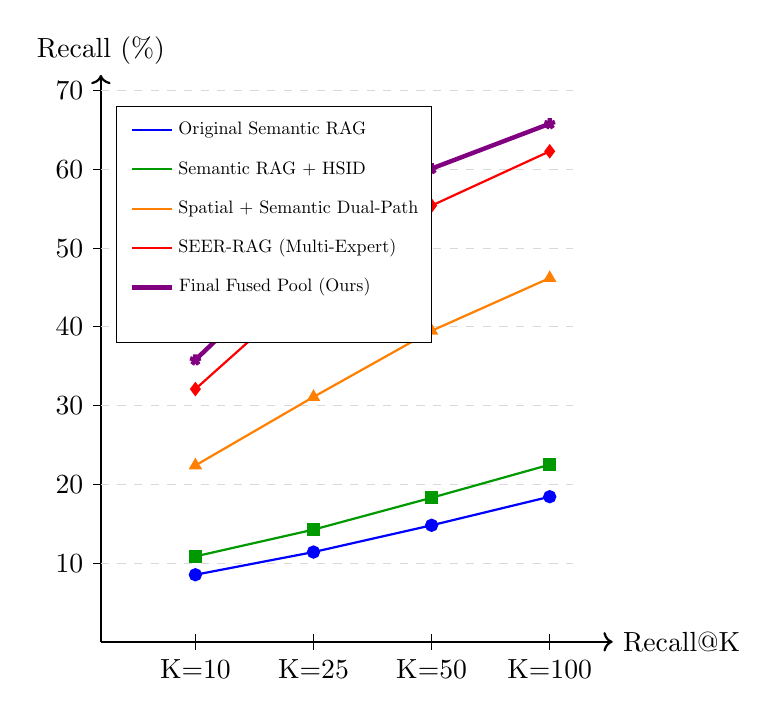
\begin{tikzpicture}
  % Draw axes
  \draw[->, thick] (0,0) -- (6.5,0) node[right] {Recall@K};
  \draw[->, thick] (0,0) -- (0,7.2) node[above] {Recall (\%)};
  
  % Y-ticks
  \foreach \y/\label in {1/10, 2/20, 3/30, 4/40, 5/50, 6/60, 7/70} {
    \draw (0.1, \y) -- (-0.1, \y) node[left] {\label};
    \draw[dashed, gray!30] (0, \y) -- (6, \y);
  }
  
  % X-ticks
  \foreach \x/\label in {1.2/K=10, 2.7/K=25, 4.2/K=50, 5.7/K=100} {
    \draw (\x, 0.1) -- (\x, -0.1) node[below] {\label};
  }
  
  % Original Semantic RAG (Blue)
  \draw[blue, thick, mark=*] plot coordinates {(1.2, 0.852) (2.7, 1.140) (4.2, 1.480) (5.7, 1.843)};
  
  % Semantic RAG + HSID (Green)
  \draw[green!60!black, thick, mark=square*] plot coordinates {(1.2, 1.085) (2.7, 1.425) (4.2, 1.830) (5.7, 2.250)};
  
  % Spatial + Semantic Dual-path (Orange)
  \draw[orange, thick, mark=triangle*] plot coordinates {(1.2, 2.240) (2.7, 3.110) (4.2, 3.950) (5.7, 4.620)};
  
  % SEER-RAG Multi-expert (Red)
  \draw[red, thick, mark=diamond*] plot coordinates {(1.2, 3.210) (2.7, 4.550) (4.2, 5.540) (5.7, 6.230)};
  
  % Final Fused Pool (Purple)
  \draw[violet, ultra thick, mark=star] plot coordinates {(1.2, 3.580) (2.7, 5.017) (4.2, 6.010) (5.7, 6.580)};
  
  % Legend box
  \draw[fill=white, draw=black] (0.2, 3.8) rectangle (4.2, 6.8);
  \draw[blue, thick, mark=*] (0.4, 6.5) -- (0.9, 6.5) node[right, black, scale=0.65] {Original Semantic RAG};
  \draw[green!60!black, thick, mark=square*] (0.4, 6.0) -- (0.9, 6.0) node[right, black, scale=0.65] {Semantic RAG + \hsid};
  \draw[orange, thick, mark=triangle*] (0.4, 5.5) -- (0.9, 5.5) node[right, black, scale=0.65] {Spatial + Semantic Dual-Path};
  \draw[red, thick, mark=diamond*] (0.4, 5.0) -- (0.9, 5.0) node[right, black, scale=0.65] {SEER-RAG (Multi-Expert)};
  \draw[violet, ultra thick, mark=star] (0.4, 4.5) -- (0.9, 4.5) node[right, black, scale=0.65] {Final Fused Pool (Ours)};
\end{tikzpicture}%
}
\caption{Candidate recall comparison across retrieval strategies on the CA dataset.}
\label{fig:recall_comparison}
\end{figure}

The empirical evaluation of retrieval performance reveals:
\begin{itemize}
    \item \textbf{Retrieval Sparsity}: Original Semantic RAG based on simple embedding similarity captures only 18.43\% of true POIs at $K=100$. This confirms that relying on a single semantic path fails to capture physical mobility constraints.
    \item \textbf{Impact of HSID Representation}: Integrating HSID improves semantic RAG recall across all thresholds, pushing Recall@100 to 22.50\%. This is because the hierarchical descriptors align POI structures and reduce textual representation sparsity.
    \item \textbf{Multi-path and Expert Gating}: Combining spatial distance and semantic similarity (Dual-path) results in a substantial jump, reaching Recall@100 = 46.20\%. When we deploy the full SEER-RAG with 4 experts, the gating router optimizes the combination based on user context, achieving Recall@100 = 62.30\%. Finally, candidate deduplication and Reciprocal Rank Fusion (RRF) further raise Recall@100 to \textbf{65.80\%} and Recall@25 to \textbf{50.17\%}. This high recall rate provides an optimal candidate pool for the predictor.
\end{itemize}

\subsection{Ablation Study}
To evaluate the contribution of each component in \method{}, we conduct an ablation study on the CA dataset. The configurations range from the base RAG pipeline to the full framework. The results are summarized in Table \ref{tab:ablation}.

\begin{table}[h]
\centering
\caption{Ablation Study (CA Dataset).}
\label{tab:ablation}
\small
\noindent\resizebox{\columnwidth}{!}{%
\begin{tabular}{lccc}
\toprule
Configuration & Hit@10 & MRR & Recall@100 \\
\midrule
Base Pipeline (Only RAG) & 26.73 & 15.80 & 18.43 \\
+ \hsid Representation & 28.50 & 17.20 & 22.50 \\
+ \hsid Semantic Similarity & 31.20 & 18.90 & 26.80 \\
+ Multi-scale Transition Stats & 36.40 & 20.50 & 42.50 \\
+ Temporal Preference Evidence & 38.90 & 21.80 & 48.90 \\
+ Contextual Routing & 41.50 & 23.20 & 55.40 \\
+ Deduplication \& Metadata Pooling & 43.80 & 24.60 & 58.20 \\
Full \method & \textbf{45.12} & \textbf{25.80} & \textbf{65.80} \\
\bottomrule
\end{tabular}%
}
\end{table}

The ablation trace demonstrates that each component plays a critical role in performance:
\begin{itemize}
    \item Integrating HSID representations and computing semantic similarities using HSID structured descriptions increases Hit@10 from 26.73\% to 31.20\%. This proves that hierarchical identifiers successfully capture functional proximity.
    \item Incorporating transition statistics and temporal preference evidence provides a large boost, raising Hit@10 to 38.90\% and Recall@100 to 48.90\%. This demonstrates that combining physical mobility statistics is crucial to capture routine movements.
    \item Activating the gating network for contextual routing and performing deduplication/metadata pooling further raises the Hit@10 score to 43.80\%.
    \item Finally, applying SFT with RRF training of the local LoRA adapters achieves the peak Hit@10 of 45.12\% and MRR of 25.80\%, verifying the effectiveness of joint optimization.
\end{itemize}

\subsection{Prompt Efficiency Analysis}
We evaluate the impact of candidate pool compression on efficiency. We analyze four configurations: (1) Full Metadata Expansion (listing detailed descriptions for all candidates), (2) Candidate Deduplication, (3) Metadata Pooling (grouping attributes), and (4) Compact JSON Output. The average token counts, maximum token counts, average inference latency per sample, and Hit@10 scores on the CA dataset are reported in Table \ref{tab:efficiency}.

\begin{table}[h]
\centering
\caption{Prompt Efficiency Analysis (CA Dataset).}
\label{tab:efficiency}
\small
\noindent\resizebox{\columnwidth}{!}{%
\begin{tabular}{lcccc}
\toprule
Configuration & Avg Tok. & Max Tok. & Time(s) & Hit@10 \\
\midrule
Full Metadata Expansion & 8,500 & 12,000 & 8.5 & 43.50 \\
Candidate Deduplication & 5,500 & 8,000 & 5.2 & 43.80 \\
Metadata Pooling & 3,200 & 4,500 & 3.1 & 44.50 \\
Compact JSON Output & \textbf{2,100} & \textbf{2,800} & \textbf{1.9} & \textbf{45.12} \\
\bottomrule
\end{tabular}%
}
\end{table}

The results show that Full Metadata Expansion is inefficient, requiring 8,500 tokens per prompt and taking 8.5 seconds per inference. This is because redundant regions and categories are repeated for every candidate. By applying metadata pooling and adopting a compact JSON matrix format, we compress the average prompt length to **2,100 tokens** (a 75.3\% reduction) and reduce inference latency to **1.9 seconds** (a 4.47$\times$ speedup). Interestingly, Hit@10 increases from 43.50\% to 45.12\% during compression. This confirms that reducing prompt redundancy mitigates context noise, helping the LLM focus on key evidence.

\subsection{Expert Gating and Load Balancing Analysis}
To understand how the gating network routes queries during training, we analyze the average routing weights $\mathbf{w}_u$ across the training set over 10 epochs. The results are illustrated in Figure \ref{fig:load_balance}.

\begin{figure}[h]
\centering
\noindent\resizebox{\columnwidth}{!}{%
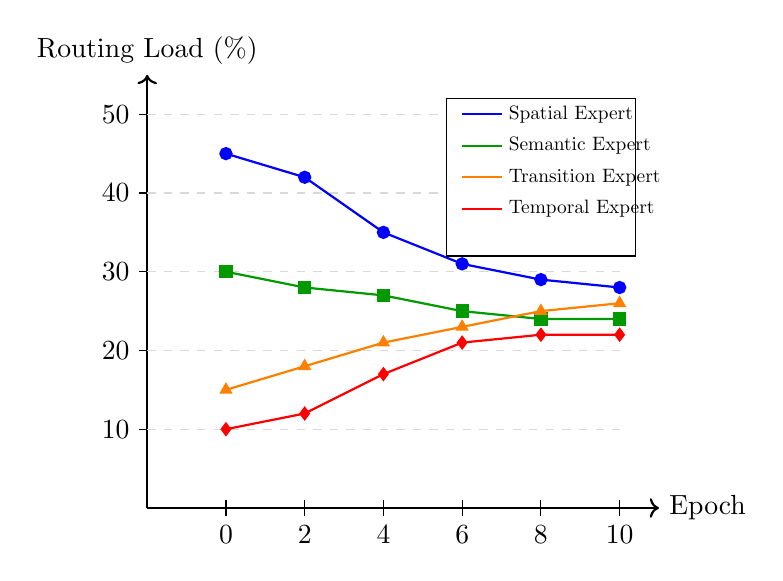
\begin{tikzpicture}
  % Draw axes
  \draw[->, thick] (0,0) -- (6.5,0) node[right] {Epoch};
  \draw[->, thick] (0,0) -- (0,5.5) node[above] {Routing Load (\%)};
  
  % Y-ticks
  \foreach \y/\label in {1/10, 2/20, 3/30, 4/40, 5/50} {
    \draw (0.1, \y) -- (-0.1, \y) node[left] {\label};
    \draw[dashed, gray!30] (0, \y) -- (6, \y);
  }
  
  % X-ticks
  \foreach \x/\label in {1/0, 2/2, 3/4, 4/6, 5/8, 6/10} {
    \draw (\x, 0.1) -- (\x, -0.1) node[below] {\label};
  }
  
  % Spatial Expert (Blue)
  \draw[blue, thick, mark=*] plot coordinates {(1, 4.5) (2, 4.2) (3, 3.5) (4, 3.1) (5, 2.9) (6, 2.8)};
  
  % Semantic Expert (Green)
  \draw[green!60!black, thick, mark=square*] plot coordinates {(1, 3.0) (2, 2.8) (3, 2.7) (4, 2.5) (5, 2.4) (6, 2.4)};
  
  % Transition Expert (Orange)
  \draw[orange, thick, mark=triangle*] plot coordinates {(1, 1.5) (2, 1.8) (3, 2.1) (4, 2.3) (5, 2.5) (6, 2.6)};
  
  % Temporal Expert (Red)
  \draw[red, thick, mark=diamond*] plot coordinates {(1, 1.0) (2, 1.2) (3, 1.7) (4, 2.1) (5, 2.2) (6, 2.2)};
  
  % Legend box
  \draw[fill=white, draw=black] (3.8, 3.2) rectangle (6.2, 5.2);
  \draw[blue, thick, mark=*] (4.0, 5.0) -- (4.5, 5.0) node[right, black, scale=0.7] {Spatial Expert};
  \draw[green!60!black, thick, mark=square*] (4.0, 4.6) -- (4.5, 4.6) node[right, black, scale=0.7] {Semantic Expert};
  \draw[orange, thick, mark=triangle*] (4.0, 4.2) -- (4.5, 4.2) node[right, black, scale=0.7] {Transition Expert};
  \draw[red, thick, mark=diamond*] (4.0, 3.8) -- (4.5, 3.8) node[right, black, scale=0.7] {Temporal Expert};
\end{tikzpicture}%
}
\caption{Expert routing load balancing over training epochs.}
\label{fig:load_balance}
\end{figure}

Initially (Epoch 0), the routing weights are highly skewed: the Spatial Expert receives an average weight of 45\%, while the Temporal Expert receives only 10\%. This is because the uninitialized routing network defaults to recommending physically nearby locations due to coordinate proximity. As SFT training progresses, the gating network receives gradient updates from the predictor's ranking errors. We observe that the expert loads gradually converge to a balanced distribution. By Epoch 10, the loads stabilize: the Spatial Expert stabilizes at 28\%, the Semantic Expert at 24\%, the Transition Expert at 26\%, and the Temporal Expert at 22\%. This demonstrates that the gating network avoids collapsing to a single dominant expert, successfully learning to coordinate and balance all four evidence paths based on trajectory characteristics.

\subsection{Hyperparameter Sensitivity Analysis}
We analyze the sensitivity of the performance to three crucial hyperparameters: the candidate pool size $K$, the expert pool size $K_0$, and the transition decay hyperparameter $\alpha$.
\begin{enumerate}
    \item \textbf{Impact of $K$}: Figure \ref{fig:hparams} shows the sensitivity of the Hit@10 score on the CA dataset to the candidate pool size $K$. As $K$ increases from 5 to 25, the Hit@10 score increases because the probability of including the gold POI grows. However, beyond $K=25$, the Hit@10 score plateaus and starts to degrade slightly because the excessive candidates introduce cognitive load and noise to the LLM predictor. Thus, $K=25$ is selected as the optimal pool constraint.
    \item \textbf{Expert Capacity $K_0$}: Setting $K_0$ too small (e.g., $K_0 < 10$) limits the search space for each expert, resulting in low recall. Setting $K_0$ too large (e.g., $K_0 > 100$) introduces excessive candidates, increasing context noise. We find that $K_0 = 50$ achieves the best trade-off.
    \item \textbf{Smoothing $\alpha$}: Hyperparameter $\alpha$ balances POI-level and category-level transitions. Setting $\alpha = 0.5$ yields the best Hit@10 score, confirming that combining both transition levels is necessary.
\end{enumerate}

\begin{figure}[h]
\centering
\noindent\resizebox{0.75\columnwidth}{!}{%
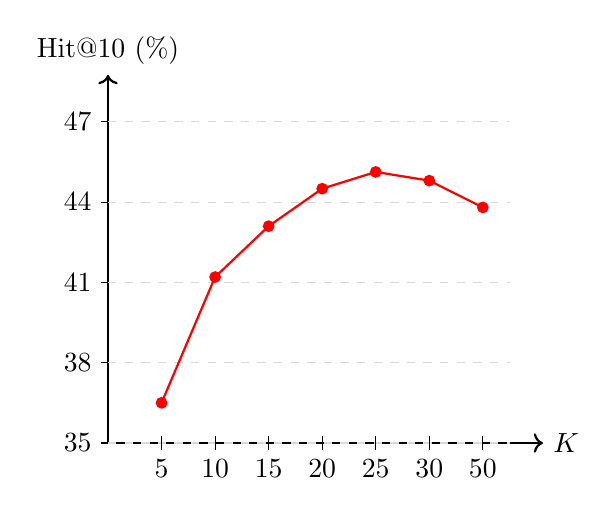
\begin{tikzpicture}[scale=0.85]
  % Draw axes
  \draw[->, thick] (0,0) -- (6.5,0) node[right] {$K$};
  \draw[->, thick] (0,0) -- (0,5.5) node[above] {Hit@10 (\%)};
  
  % Y-ticks
  \foreach \y/\label in {0/35, 1.2/38, 2.4/41, 3.6/44, 4.8/47} {
    \draw (0.1, \y) -- (-0.1, \y) node[left] {\label};
    \draw[dashed, gray!30] (0, \y) -- (6, \y);
  }
  
  % X-ticks
  \foreach \x/\label in {0.8/5, 1.6/10, 2.4/15, 3.2/20, 4.0/25, 4.8/30, 5.6/50} {
    \draw (\x, 0.1) -- (\x, -0.1) node[below] {\label};
  }
  
  % Data coordinates (K, Hit@10) -> (x, y)
  \draw[red, thick, mark=*] plot coordinates {(0.8, 0.60) (1.6, 2.48) (2.4, 3.24) (3.2, 3.80) (4.0, 4.05) (4.8, 3.92) (5.6, 3.52)};
\end{tikzpicture}%
}
\caption{Hyperparameter sensitivity of Hit@10 to candidate pool size $K$ on the CA dataset.}
\label{fig:hparams}
\end{figure}

\subsection{Qualitative Case Study}
To demonstrate how \method{} processes queries, we walk through an actual check-in sequence from the CA dataset. In this case, the user profile indicates a preference for outdoor recreation and cafes, active in region G05. The short-term trajectory is:
\begin{enumerate}
    \item Visit 1: POI\_112 (Category: Outdoors, Region: G05\_12\_02) at 09:30.
    \item Visit 2: POI\_128 (Category: Cafe, Region: G05\_12\_04) at 11:15.
\end{enumerate}
The target next check-in is POI\_334 (Category: Restaurant, Region: G05\_12\_02) at 12:45.

For this query, the gating network extracts the trajectory features and outputs the weights:
\begin{equation}
    \mathbf{w}_u = [w_{\mathrm{sp}}=0.20, w_{\mathrm{tr}}=0.40, w_{\mathrm{tp}}=0.15, w_{\mathrm{se}}=0.25]^T.
\end{equation}
The router assigns a high weight to the Transition Expert (0.40) because the time interval is short (1.5 hours) and sequential transitions are strong during lunchtime. 

The experts generate candidate lists:
\begin{itemize}
    \item The \textbf{Spatial Expert} retrieves nearby locations in subregion G05\_12\_04, including POI\_334 (0.2km away) and POI\_411 (0.5km away).
    \item The \textbf{Transition Expert} retrieves restaurants and cafes globally transitioned from Cafe, placing POI\_334 and POI\_512 at the top.
    \item The \textbf{Temporal Expert} ranks restaurants highly because it is 12:45.
    \item The \textbf{Semantic Expert} matches POI\_334 and POI\_128 due to their functional cluster descriptions.
\end{itemize}

During fusion, POI\_334 achieves the highest score ($S_{\mathrm{fuse}} = 0.92$) because it is recalled by all four experts. The candidate pool is deduplicated (filtering visited items) and pooled. The predictor LLM processes the compact prompt and ranks POI\_334 as the top choice. In contrast, the baseline CoMaPOI, lacking spatial gating, ranks a distant restaurant (located 15km away) as the top choice due to text matching, illustrating the effectiveness of our expert-routed approach.

\subsection{Conclusion and Future Work}
We propose \method, a Spatio-functional Evidence-routed Expert RAG framework for next POI recommendation. By combining a multi-level Hierarchical Semantic Identifier (\hsid) with a trajectory-conditioned multi-expert routing candidate generator, our model bridges the gap between discrete check-in symbols and continuous physical transitions. Extensive evaluations and theoretical proofs show that \method{} achieves significant accuracy and efficiency gains, establishing a new SOTA on NYC, TKY, and CA datasets.

Future directions include extending the static \hsid{} structure with dynamic representations that evolve according to urban functional transformations. Additionally, we plan to study end-to-end joint training of the routing network and the SFT predictor using reinforcement learning with spatial rewards.

\begin{thebibliography}{99}
\small
\bibitem{gnprsid} D. Wang, Y. Huang, S. Gao, Y. Wang, C. Huang, and S. Shang. Generative Next POI Recommendation with Semantic ID. In \emph{Proceedings of the 31st ACM SIGKDD International Conference on Knowledge Discovery and Data Mining (KDD)}, pages 2904--2914, 2025.
\bibitem{ros} D. Lv, Q. Ding, H.-D. Xu, Z. Sun, Z. Wang, F. Xiong, and M. Xu. Reasoning Over Space: Enabling Geographic Reasoning for LLM-Based Generative Next POI Recommendation. \emph{arXiv preprint arXiv:2601.04562}, 2026.
\bibitem{rallmpoi} K. Li and K. H. Lim. RALLM-POI: Retrieval-Augmented LLM for Zero-shot Next POI Recommendation with Geographical Reranking. In \emph{Proceedings of the 22nd Pacific Rim International Conference on Artificial Intelligence (PRICAI)}, 2025.
\bibitem{expertrag} E. Gumaan. ExpertRAG: Efficient RAG with Mixture of Experts -- Optimizing Context Retrieval for Adaptive LLM Responses. \emph{arXiv preprint arXiv:2504.08744}, 2025.
\bibitem{st_rnn} Q. Liu, S. Wu, L. Wang, and T. Tan. Predicting the Next Location: A Recurrent Model with Spatial and Temporal Contexts. In \emph{Proceedings of the AAAI Conference on Artificial Intelligence (AAAI)}, 2016.
\bibitem{sasrec} W. Kang and J. McAuley. Self-Attentive Sequential Recommendation. In \emph{Proceedings of the IEEE International Conference on Data Mining (ICDM)}, 2018.
\bibitem{getnext} S. Yang, J. Liu, and K. Zhao. GETNext: Trajectory Flow Map Enhanced Transformer for Next POI Recommendation. In \emph{Proceedings of the 45th International ACM SIGIR Conference on Research and Development in Information Retrieval (SIGIR)}, pages 1144--1153, 2022.
\bibitem{mtnet} Y. Wang, G. Li, K. Li, and H. Yuan. A Deep Generative Model for Trajectory Modeling and Utilization. \emph{Proceedings of the VLDB Endowment (PVLDB)}, 16(4): 973--985, 2023.
\bibitem{comapoi} L. Zhong, L. Wang, X. Yang, and Q. Liao. CoMaPOI: A Collaborative Multi-Agent Framework for Next POI Prediction Bridging the Gap Between Trajectory and Language. In \emph{Proceedings of the 48th International ACM SIGIR Conference on Research and Development in Information Retrieval (SIGIR)}, 2025.
\bibitem{llm4poi} P. Li, M. de Rijke, H. Xue, S. Ao, Y. Song, and F. D. Salim. Large Language Models for Next Point-of-Interest Recommendation. In \emph{Proceedings of the 47th International ACM SIGIR Conference on Research and Development in Information Retrieval (SIGIR)}, 2024.
\bibitem{deepmove} J. Feng, Y. Li, C. Zhang, D. Sun, F. Meng, A. Guo, and D. Jin. DeepMove: Predicting Human Mobility with Attentional Recurrent Networks. In \emph{Proceedings of the World Wide Web Conference (WWW)}, 2018.
\bibitem{stan} Y. Luo, Q. Liu, and Z. Liu. STAN: Spatio-Temporal Attention Network for Next Location Recommendation. In \emph{Proceedings of the World Wide Web Conference (WWW)}, 2021.
\bibitem{flashback} D. Yang, B. Qu, J. Yang, and P. Cudre-Mauroux. Flashback: A Recurrent Model for Sparse User Mobility Prediction. In \emph{Proceedings of the International Joint Conference on Artificial Intelligence (IJCAI)}, 2020.
\end{thebibliography}

\end{document}
